\chapter{泥岩流变数值模拟研究}
岩土工程研究的核心问题即变形与稳定性评价。工程扰动造成边坡应力场及位移场发生变化,在流变作用下位移随时间有不同程度的发展。过大的变形将导致其上构筑物受力变形的改变,影响构筑物正常工作运营,甚至造成构筑物破坏。因此,对大型岩土工程项目,分析其岩土体变形发展趋势,对工程稳定性进行评价具有重要意义。





\section{数值模型}

取江苏金坛某一长轴为\SI{70}{m},短轴为\SI{30}{m}的椭球形溶腔为研究对象进行二维测试。根据王贵君\cite{王贵君2003盐岩层中天然气存储洞室围岩长期变形特征}的研究表明,模型宽度为腔\num{5}倍以上时候,边界效应对围岩的影响可忽略不计。因此取试算模型宽度为\SI{400}{m}。为提高计算效率,故取溶腔一半进行计算,模型简图如图~\ref{jiantu}~所示。对模型进行有限元计算单元网格划分,共划分\num{3202}个单元,\num{3325}个节点,如图~\ref{jiantu}~所示。


\begin{figure}[ht!]
    \centering
    \subfigure[二维模型简图]
    {
        \begin{minipage}{7cm}
            \centering
            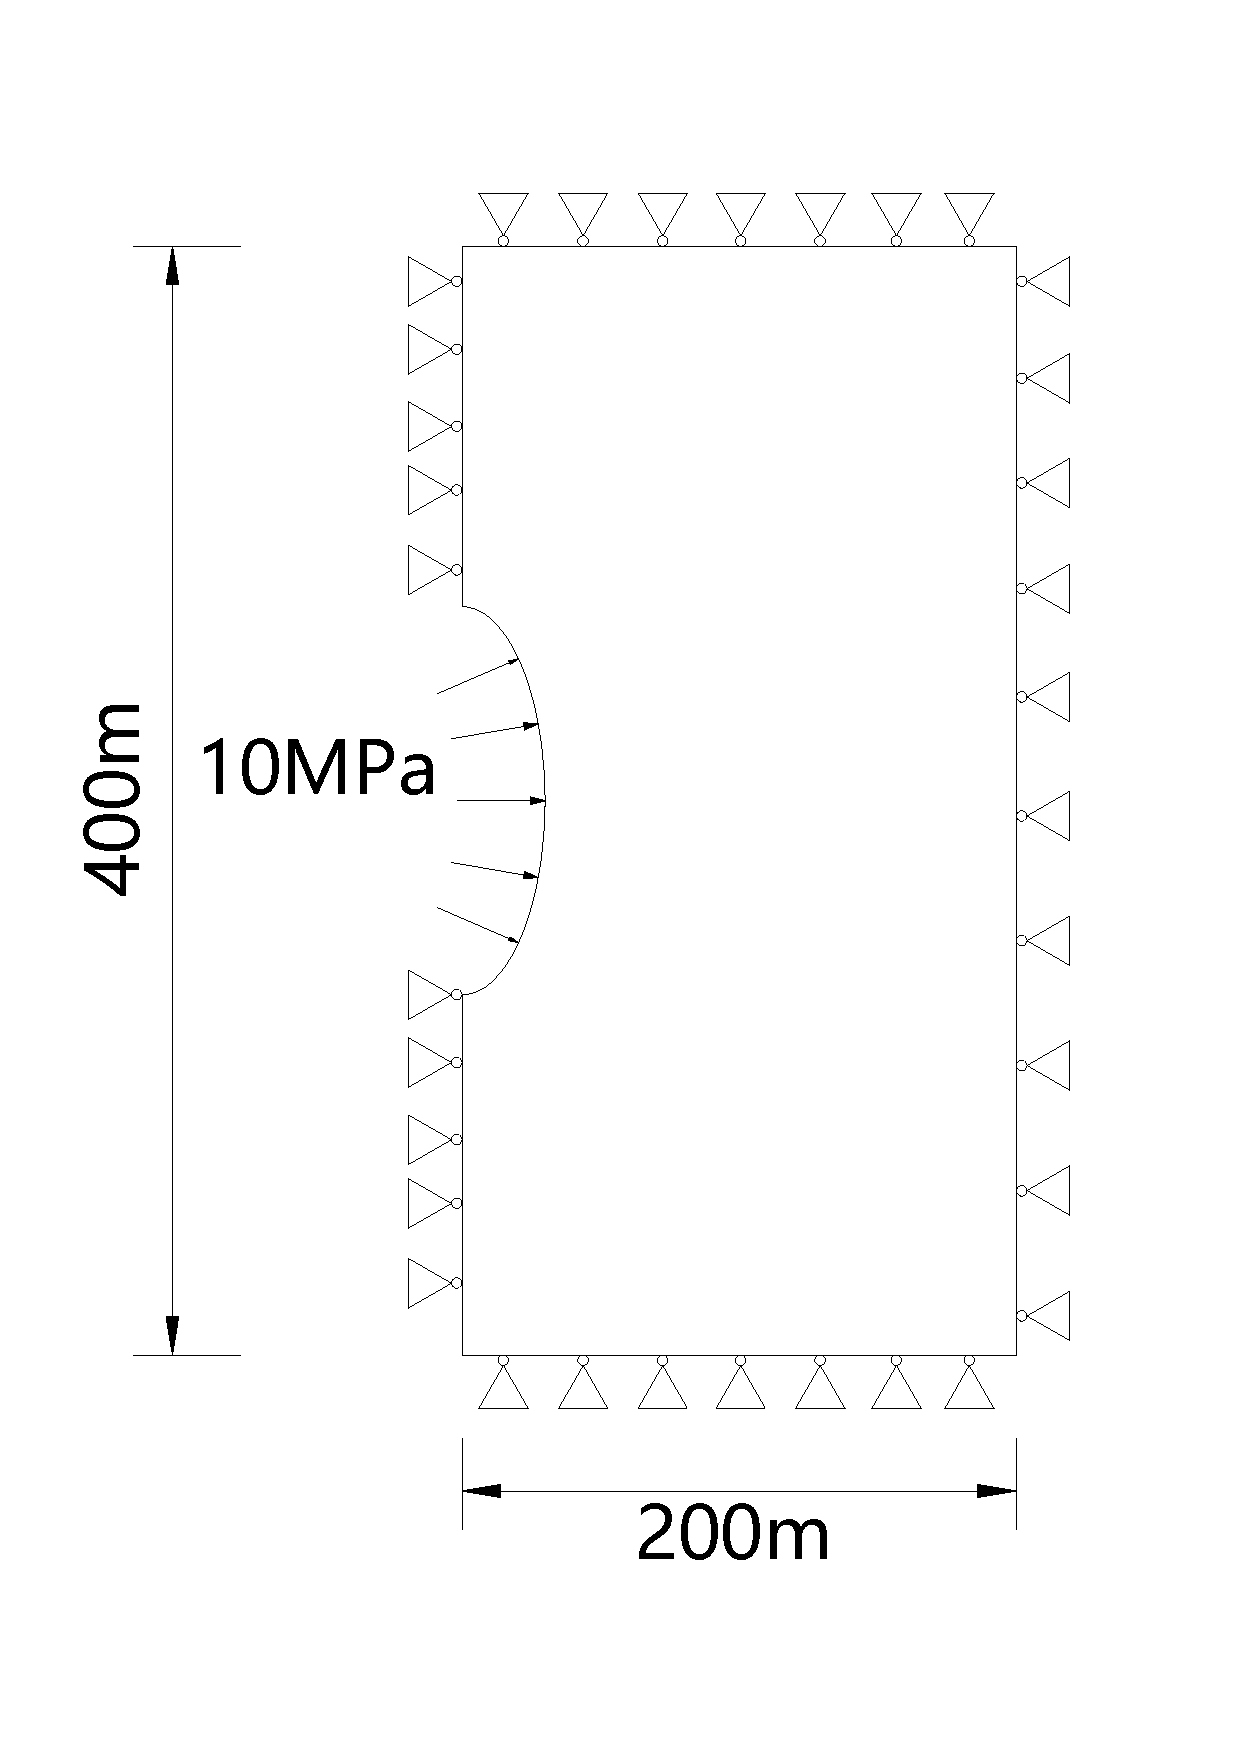
\includegraphics[width=0.95\textwidth]{img/chap4/计算模型简图.pdf}
        \end{minipage}
    }
    \subfigure[二维模型网格划分图]
    {
        \begin{minipage}{7cm}
            \centering
            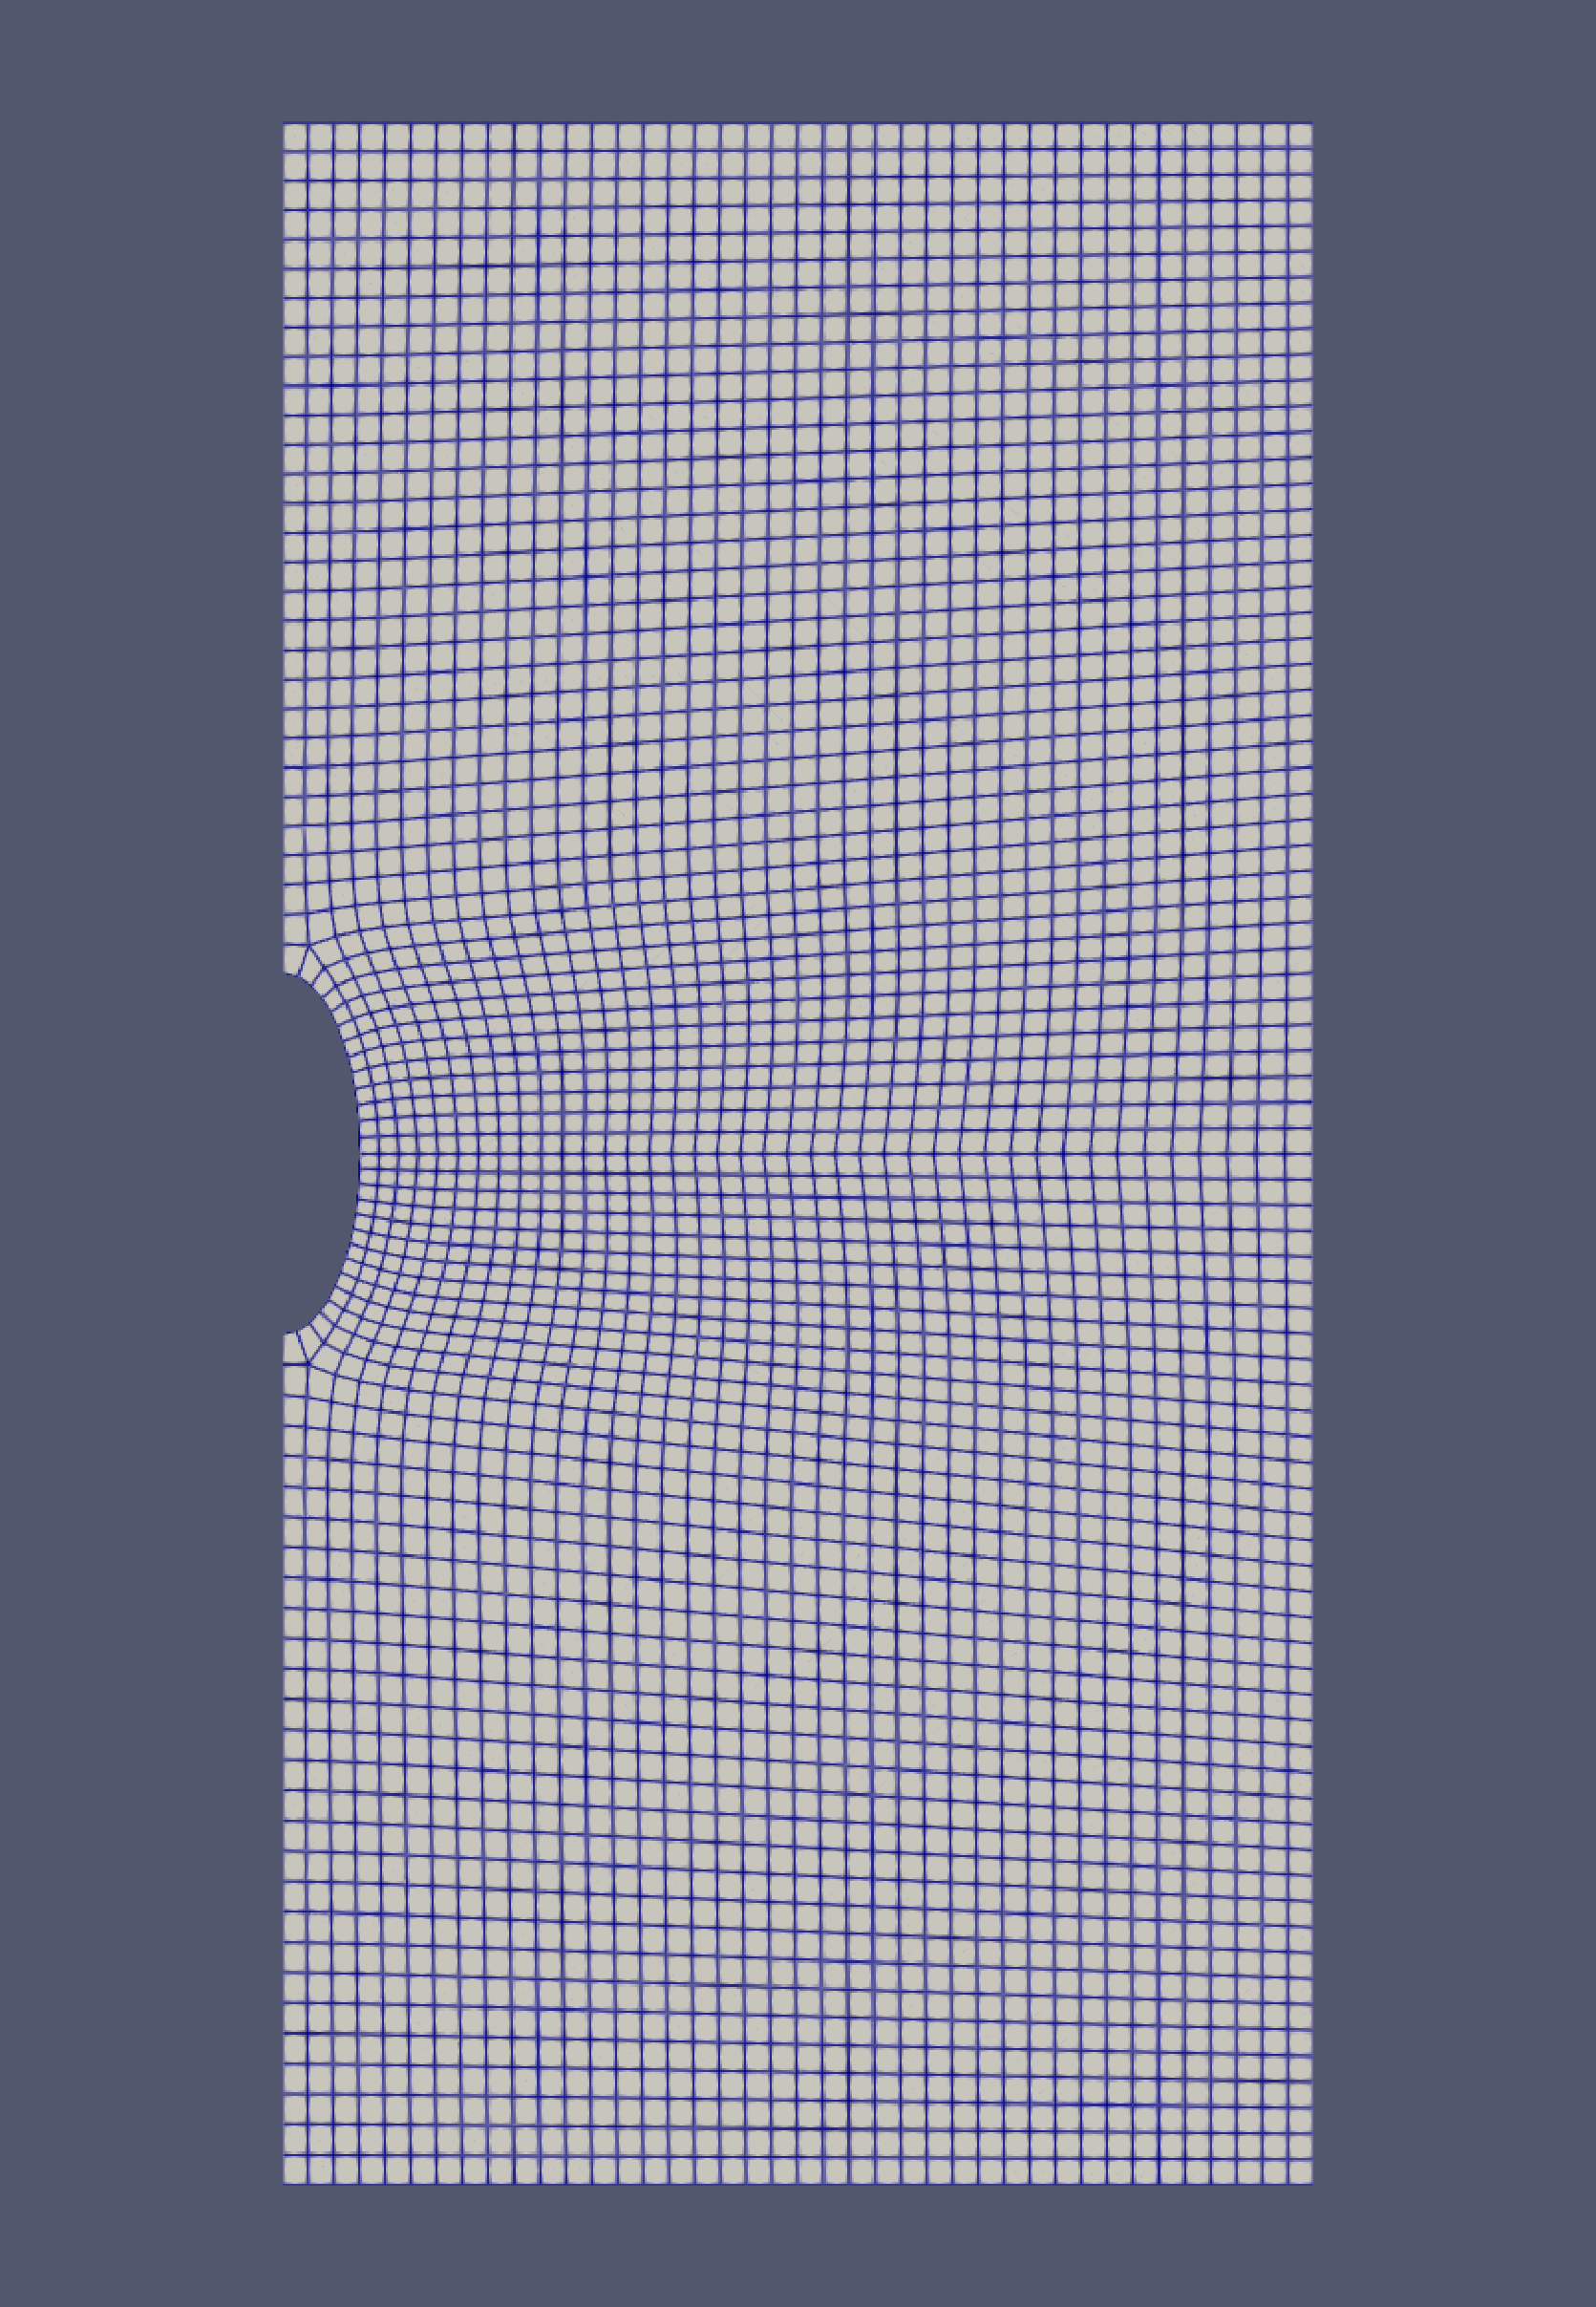
\includegraphics[width=0.95\textwidth]{img/chap4/2dmoxing.pdf}
        \end{minipage}
    }
    \caption{二维试算模型简图及网格图}
    \label{jiantu}
\end{figure}

\section{初始条件和边界条件}
计算模型的尺寸、边界等信息见图~\ref{jiantu}。

\begin{enumerate}
    \item 地应力
    
    根据马林建等\cite{马林建2009深部盐岩含夹层地层初始地应力场模拟分析}对深部盐岩自重应力分布的模拟计算结果,随着时间的增加,下底层侧压力系数不断增大,岩层越深增大的幅度越大,并趋近于$1$。本文中计算所取溶腔中心处于地下\SI{1000}{m}深处,取侧压系数$\lambda$=1,即地应力状态按照静水应力状态考虑。侧压系数$\lambda$指某点最大水平应力和垂直主应力的比值,或用两个水平应力的平均值与垂直应力的比值表示。
    %沿深度方向设置应力梯度,梯度大小为各岩层容重。

    \item 边界条件

    模型的上表面无应力边界条件;模型下表面用Y向简支约束,四周表面受相应法线方向上的简支约束,即认为模型左、右面及下端面以外的地质体为刚性体,不允许其产生法向移动,溶腔对它们的影响可以忽略。

    \item 温度条件

    模型顶端设置固定温度,为\SI{20}{\celsius} ,温度梯度为\SI{13}{\celsius/km},即围岩初始温度为\SI{33}{\celsius}。溶腔内初始压力为\SI{10}{MPa}。计算过程中温度和压力均保持不变。
\end{enumerate}

\section{模型参数}\label{section:modelparameters}
计算采用RGBa蠕变本构模型,根据金坛盐岩实验结果数据,选定相关参数如表\ref{tab:1}所示。盐岩基本力学参数及热工计算基本物理参数如表\ref{tab:2}-表\ref{tab:3}所示。

\begin{table}[ht!]\small
    \centering
    \begin{tabularx}{\textwidth}{C{1.0}C{1.0}C{1.0}C{1.0}C{1.0}}
        \toprule
        岩层 & A ($\rm{d^{-1}}$) & Q(kJ/mol) & R (kJ/mol) & m \\
        \midrule
        盐岩 & $1.336×10^{-6}$   & 15900     & 8.3143     & 5 \\ \bottomrule
    \end{tabularx}
    \caption{盐岩RGBa模型参数}
    \label{tab:1}
\end{table}

\begin{table}[ht!]\small
    \centering
    \begin{tabularx}{\textwidth}{C{1.0}C{1.0}C{1.0}C{1.0}}
        \toprule
        岩层 & 弹性模量(GPa) & 泊松比  & 密度($\rm{kg/m^3}$) \\
        \midrule
        盐岩 & 18        & 0.27 & 2310              \\
        \bottomrule
    \end{tabularx}
    \caption{盐岩基本力学参数}
    \label{tab:2}
\end{table}

\begin{table}[ht!]\small
    \centering
    \begin{tabularx}{\textwidth}{C{0.5}C{1.5}C{1.0}C{1.0}}
        \toprule
        岩层 & 导热系数($\rm{W/(m \cdot K}$)) & 比热($\rm{J/(kg\cdot K)}$) & {热膨胀系数($\rm{10^{-6}/K}$)}  \\
        \midrule
        盐岩 & 5.875         & 861                           & \num{1.2e-5} \\ \bottomrule
    \end{tabularx}
    \caption{盐岩热力学参数}%\todoiZN{热膨胀系数有单位吧}
    \label{tab:3} 
\end{table}

\section{二维模型验证}

\subsection{位移场分析}

当围岩温度分别为\SI{35}{\celsius}、\SI{90}{\celsius}、\SI{150}{\celsius}时,位移云图如~\ref{weiyiyuntu}~所示。位移在溶腔顶部和底部较小,主要集中于溶腔腰部。为分析岩体流变变形,移除最初卸荷产生的弹性形变后,绘制溶腔腰部流变最大值处位移与时间的变化关系曲线,见图~\ref{dispalment-t}。由图可知,岩体在\numrange{0}{20}天内处于初始蠕变阶段,蠕变速率较大,20天以后处于稳态蠕变阶段,蠕变速率趋于平缓。温度为\SI{35}{\celsius}时,位移最大值为\SI{0.044}{m};温度为\SI{90}{\celsius}时,位移最大值为\SI{0.047}{m};温度为\SI{150}{\celsius}时,位移最大值为\SI{0.050}{m}。由二维模型试算可得:(1)围岩温度越高产生流变越大;(2)腔体内缩,且位移主要集中于腔腰部分;(3)应力主要集中于腔顶和腔底。试算结果符合盐岩蠕变的温度效应规律和椭球型腔体的实际破坏情况。

\begin{figure}[ht!]
    \centering
    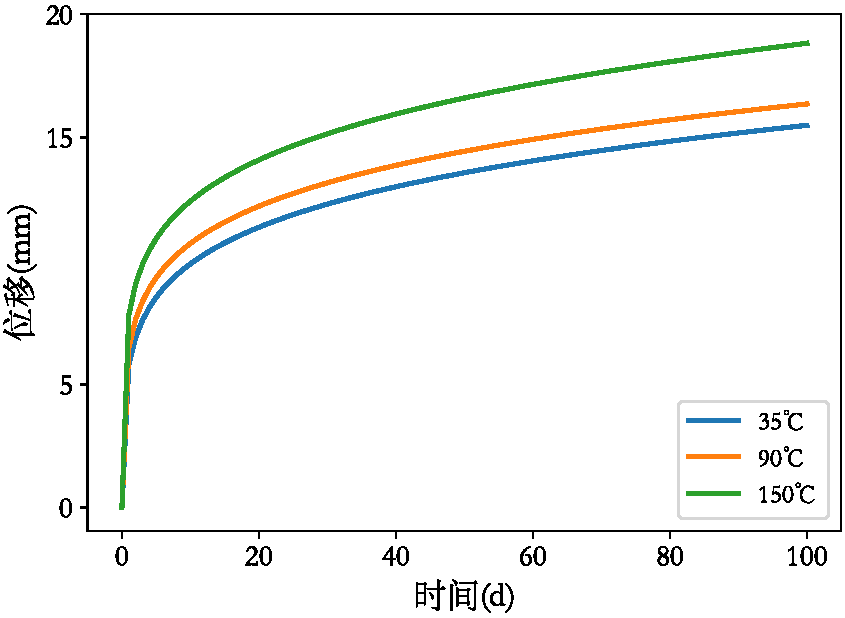
\includegraphics[width=0.55\textwidth]{img/chap4/不同温度(35℃、90℃、150℃)位移与时间曲线图.pdf}
    \caption{不同温度(35℃、90℃、150℃)位移与时间曲线图}
    \label{dispalment-t}
\end{figure}

\begin{figure}[ht!]
    \centering

    \subfigure[35℃位移云图]
    {
        \begin{minipage}{7cm}
            \centering
            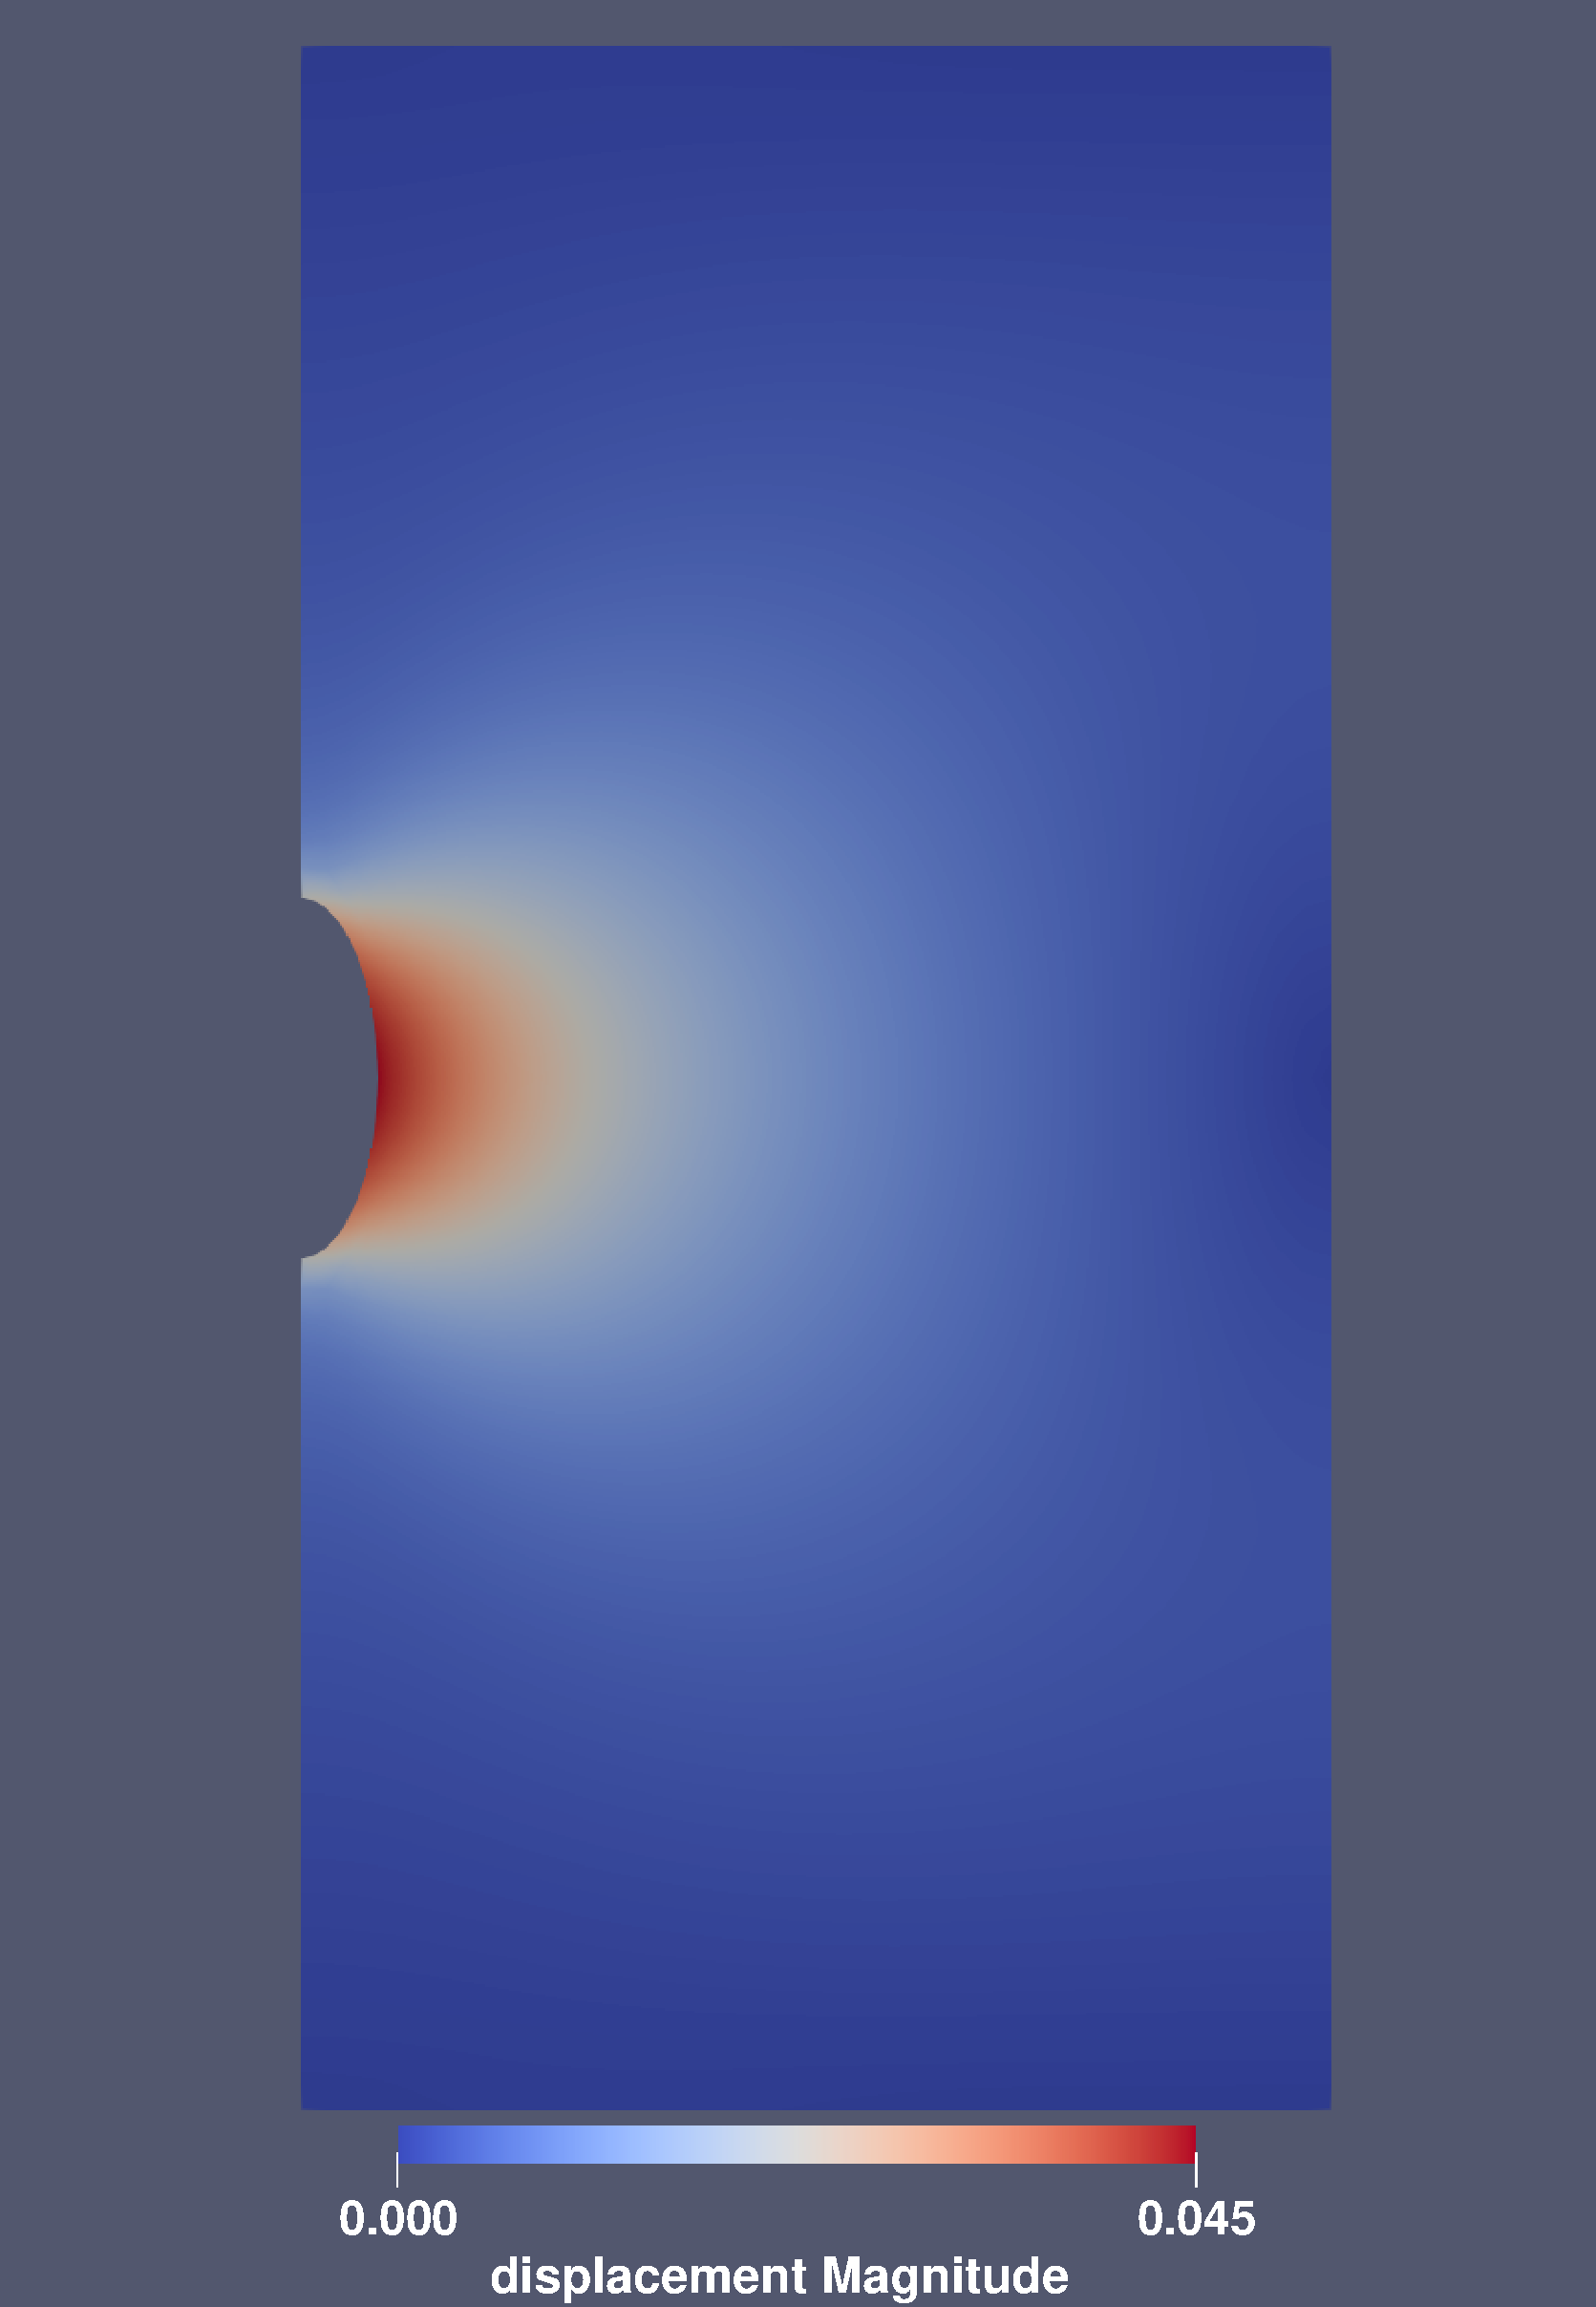
\includegraphics[width=0.95\textwidth]{img/chap4/35weiyi.pdf}
        \end{minipage}
    }
    \subfigure[90℃位移云图]
    {
        \begin{minipage}{7cm}
            \centering
            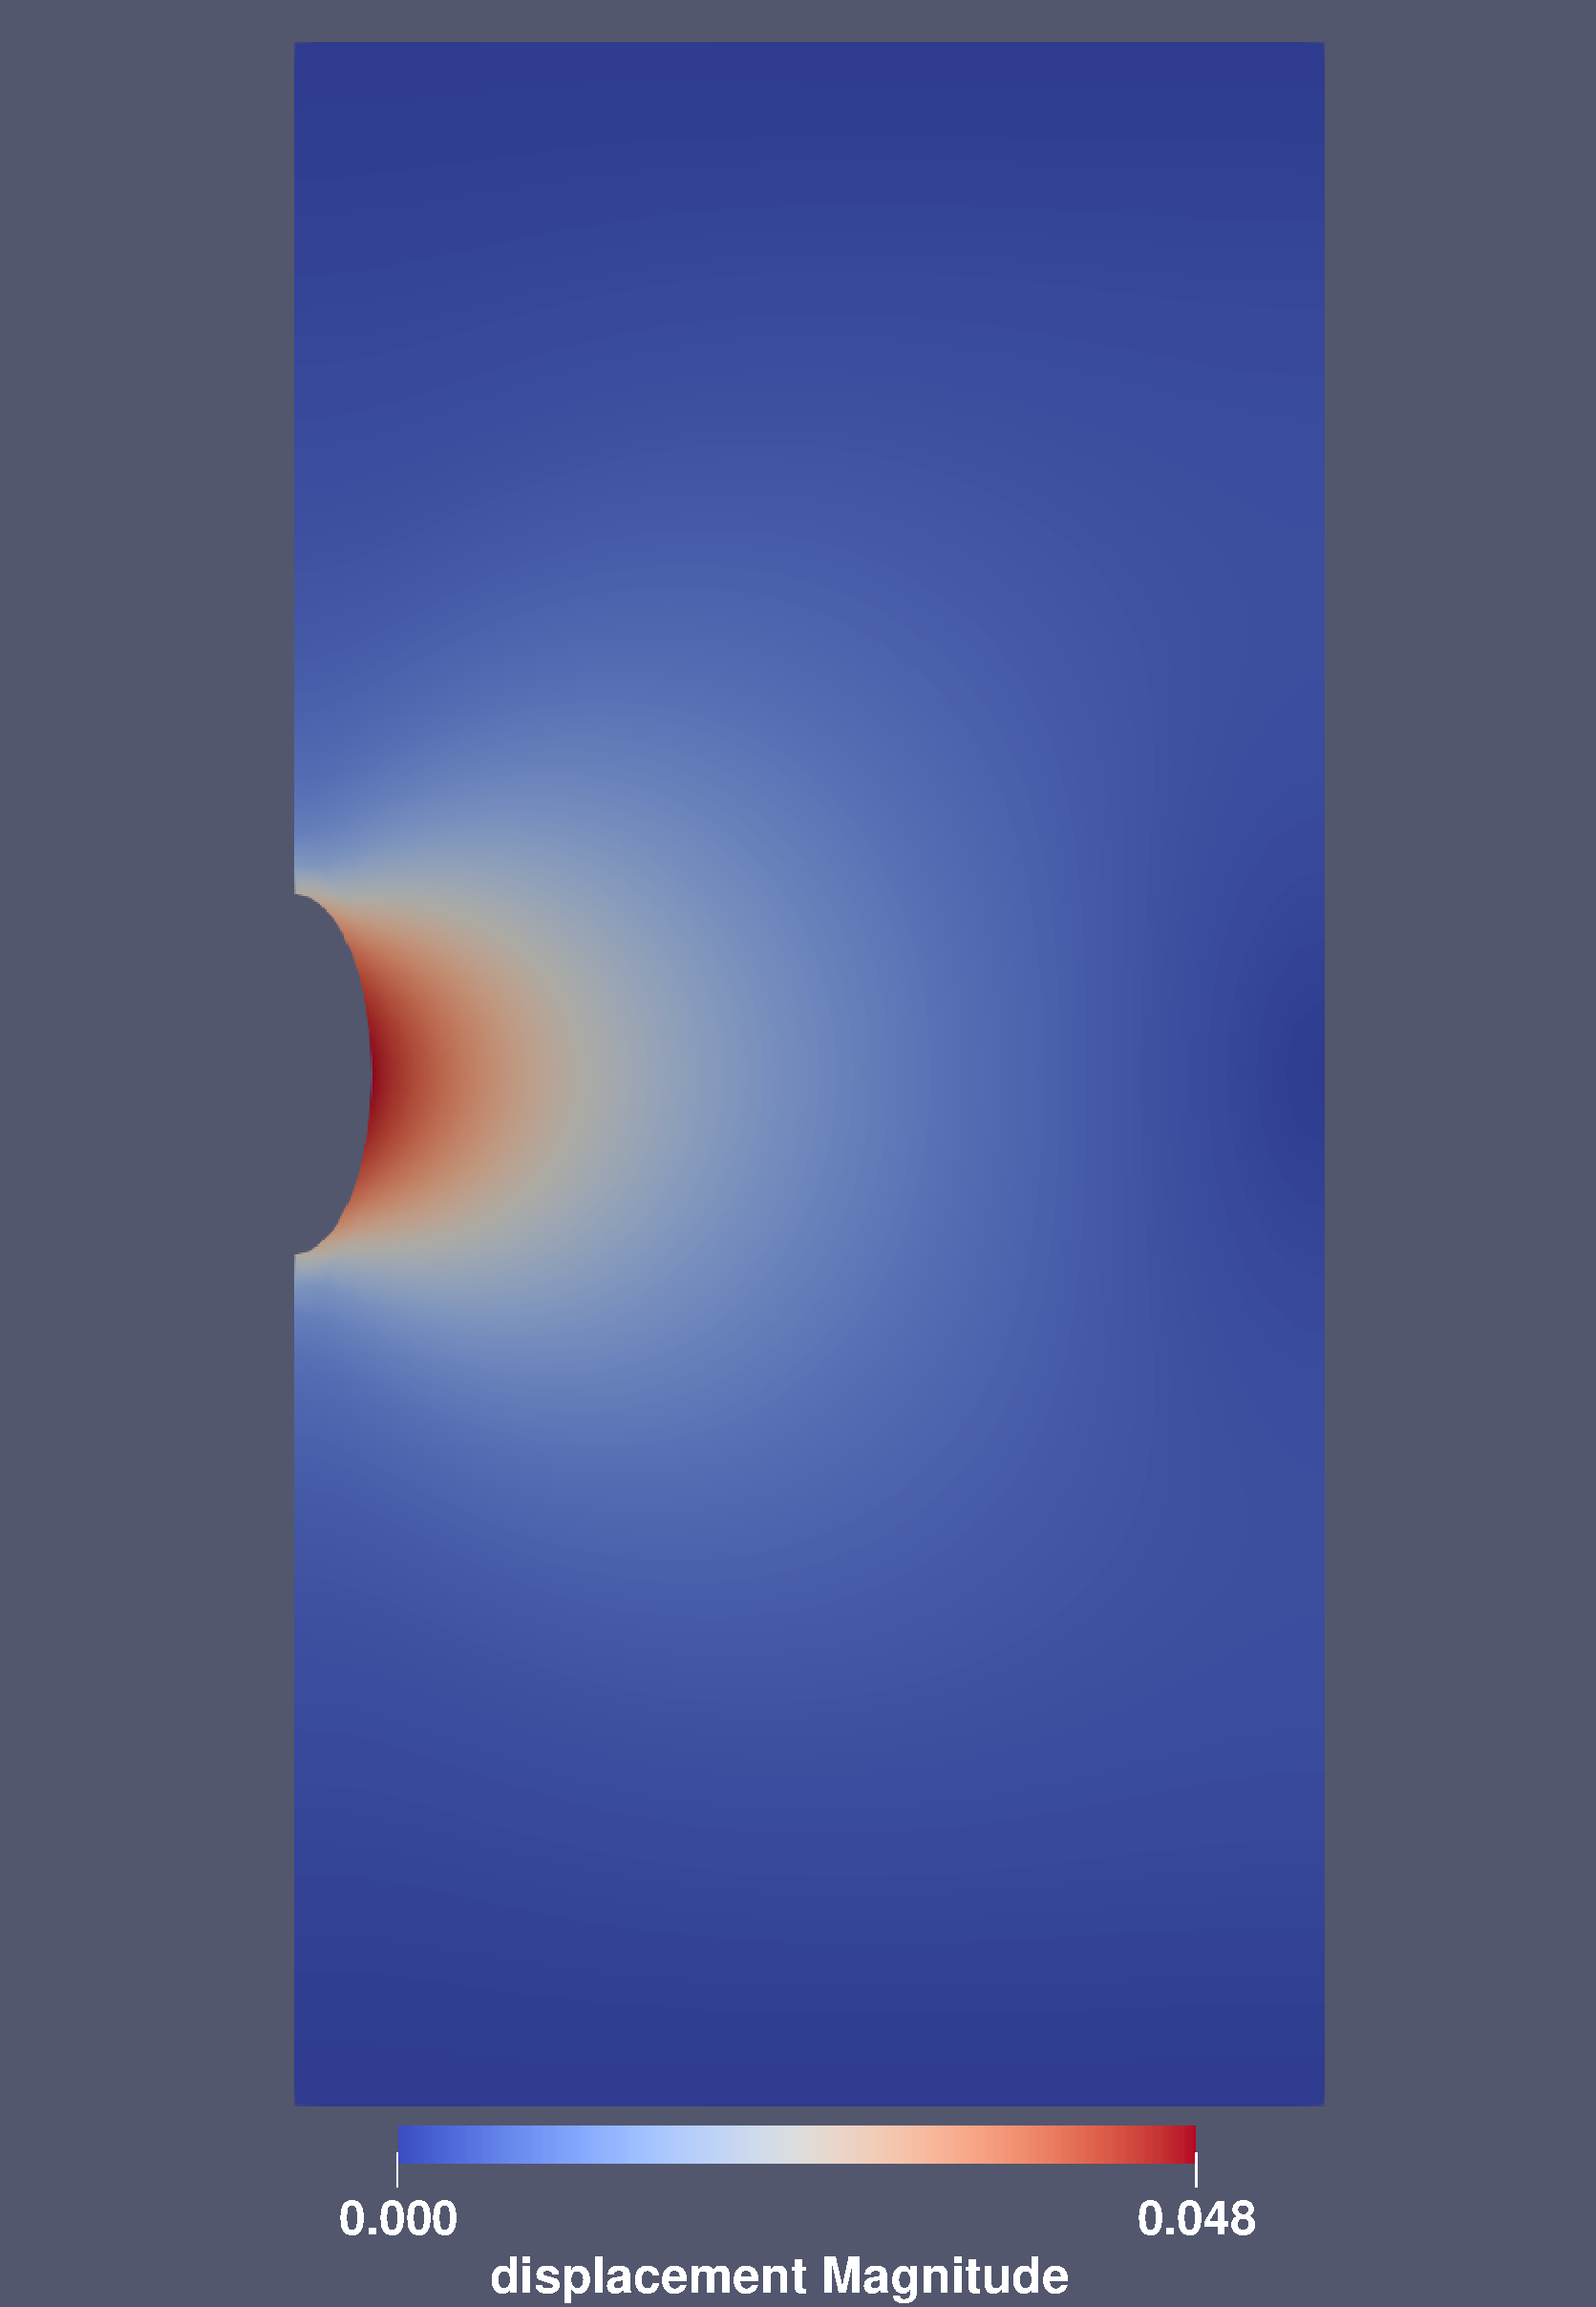
\includegraphics[width=0.95\textwidth]{img/chap4/90weiyi.pdf}
        \end{minipage}
    }
    \subfigure[150℃位移云图]
    {
        \begin{minipage}{7cm}
            \centering
            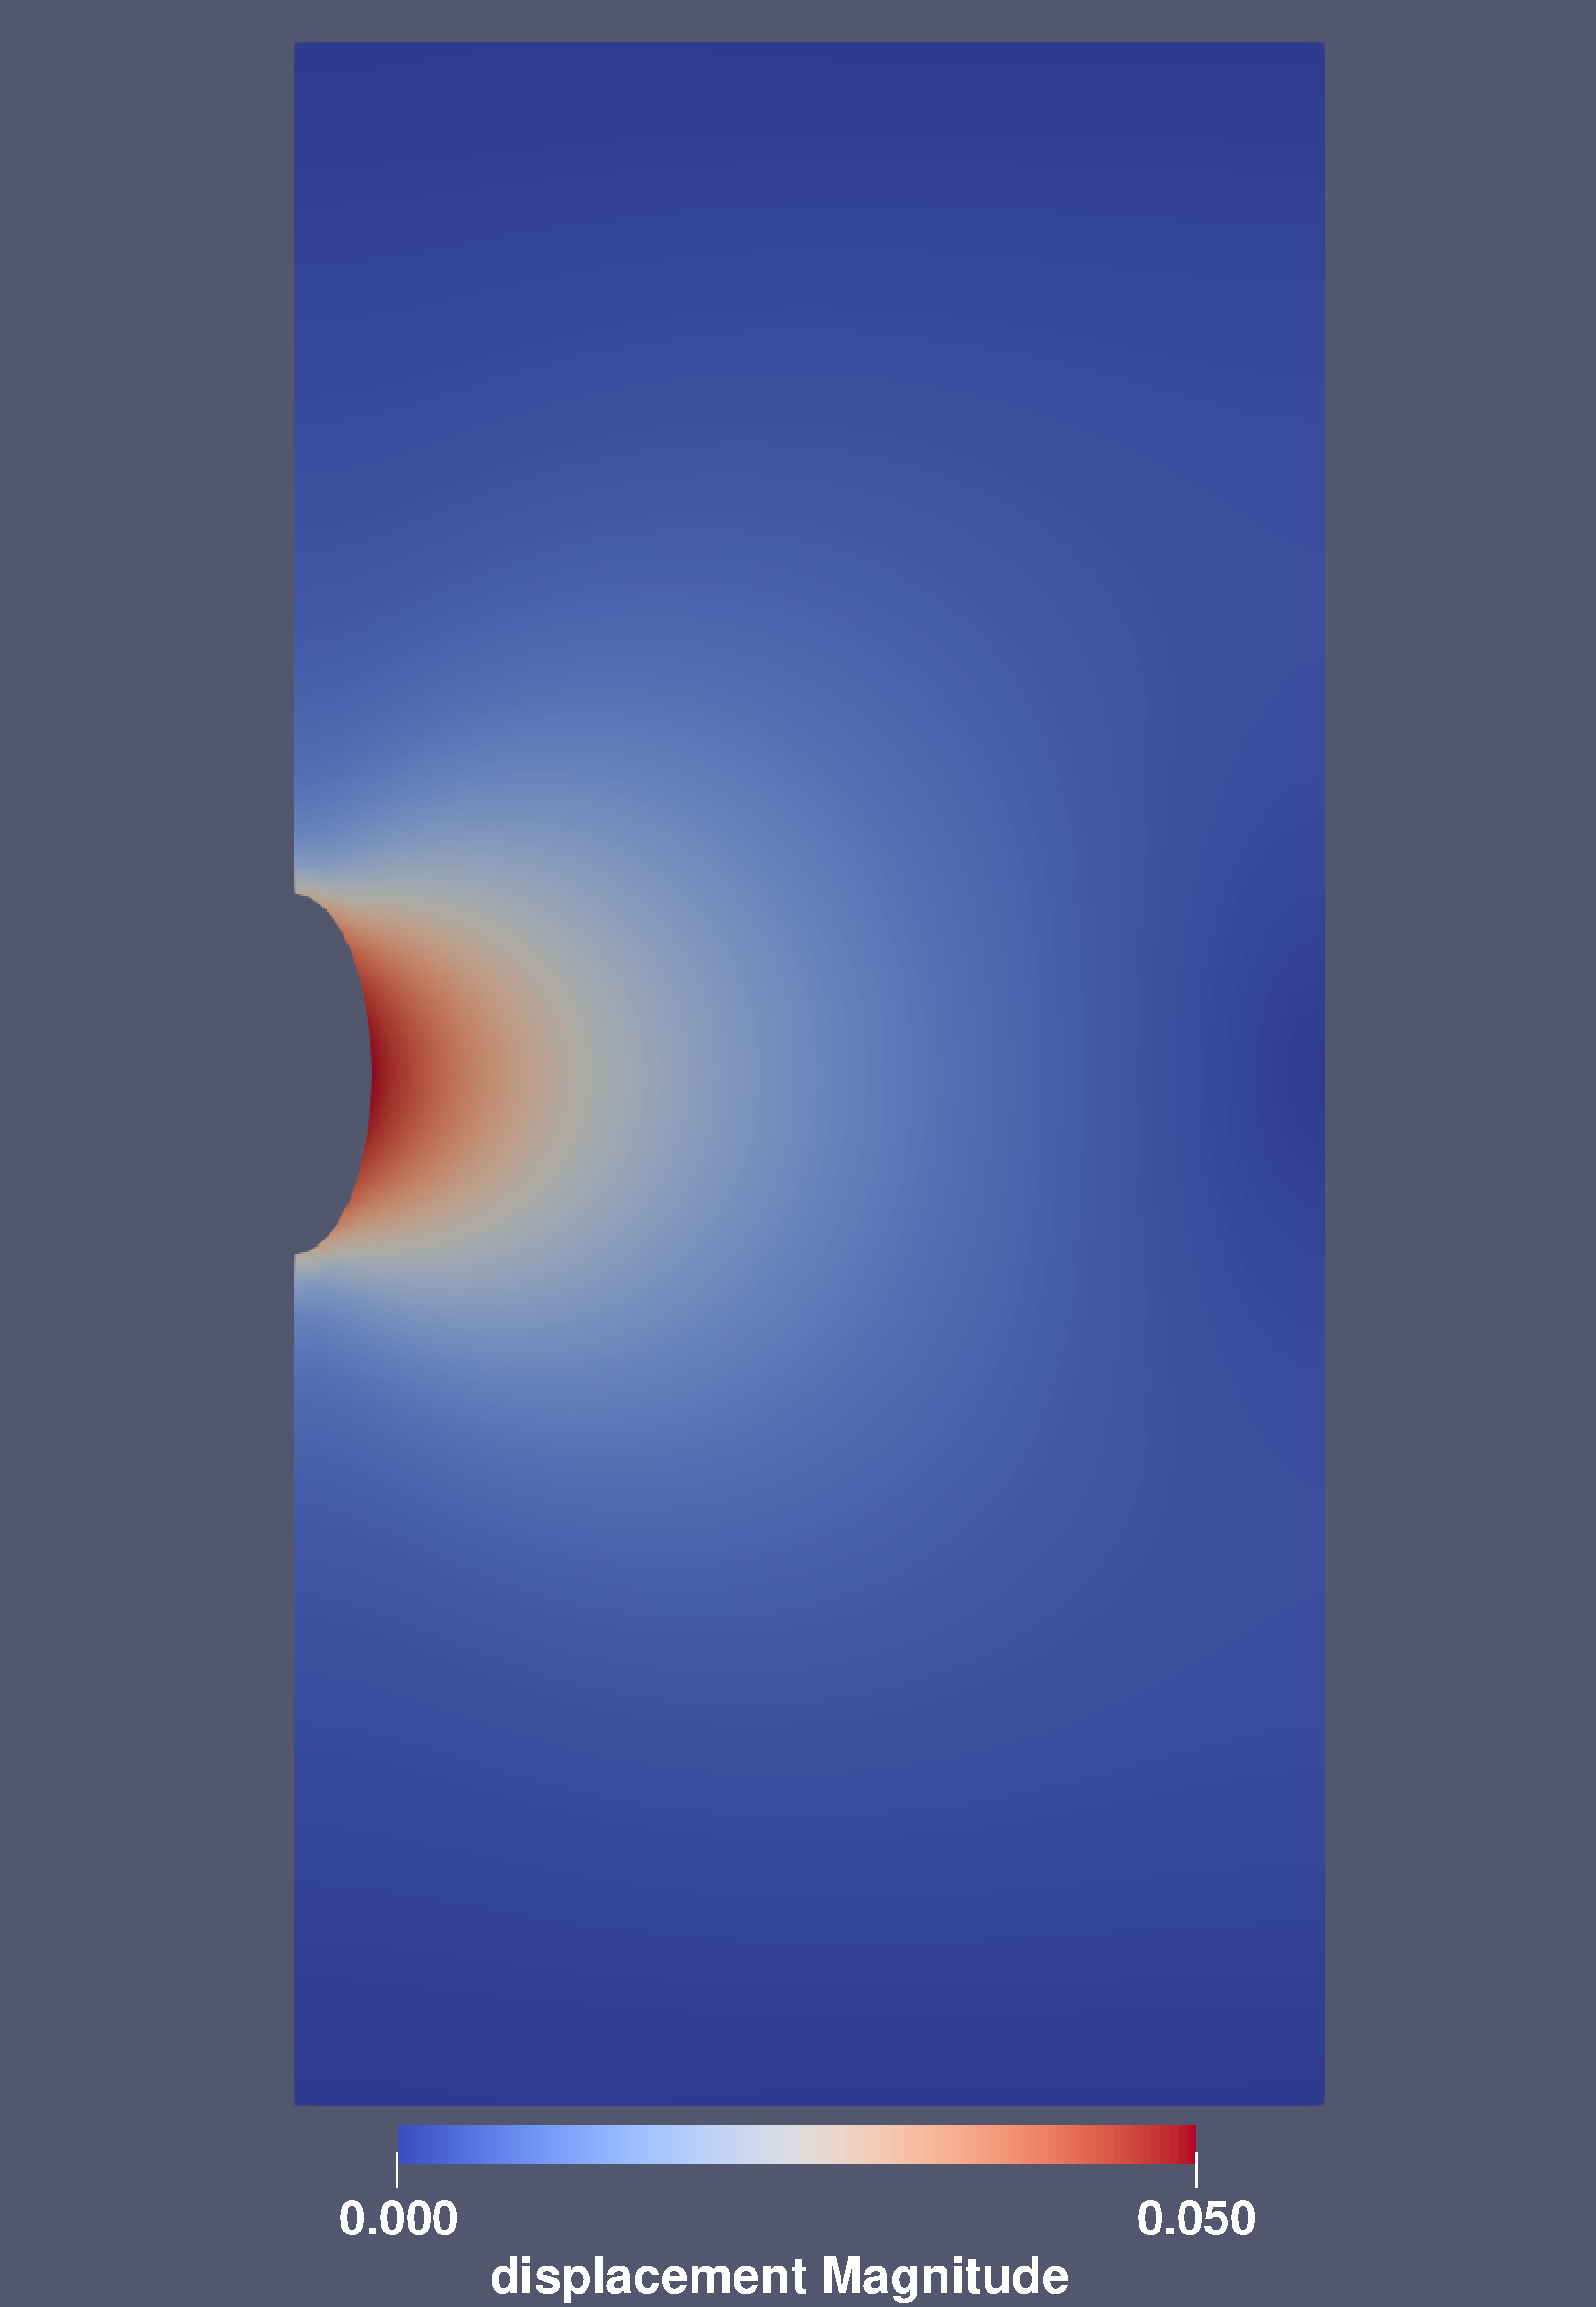
\includegraphics[width=0.95\textwidth]{img/chap4/150weiyi.pdf}
        \end{minipage}
    }
    \caption{不同温度下位移云图(单位:m)}
    \label{weiyiyuntu}
\end{figure}




\subsection{应力场分析}

由图~\ref{fig:Mises}不同温度下的Mises应力云图可以看出,溶腔在卸载后应力会发生重分布,在腔体顶部和腔体底部会形发生力集中现象。当温度为\SI{35}{\celsius}、\SI{90}{\celsius}、\SI{150}{\celsius}时,最大Mises应力分别为\SI{4}{MPa}、\SI{3.4}{MPa}、\SI{3.0}{MPa}。温度越高,最大Mises应力越小。


\begin{figure}[ht!]
    \centering
    \subfigure[35℃~Mises应力云图]
    {
        \begin{minipage}{7cm}
            \centering
            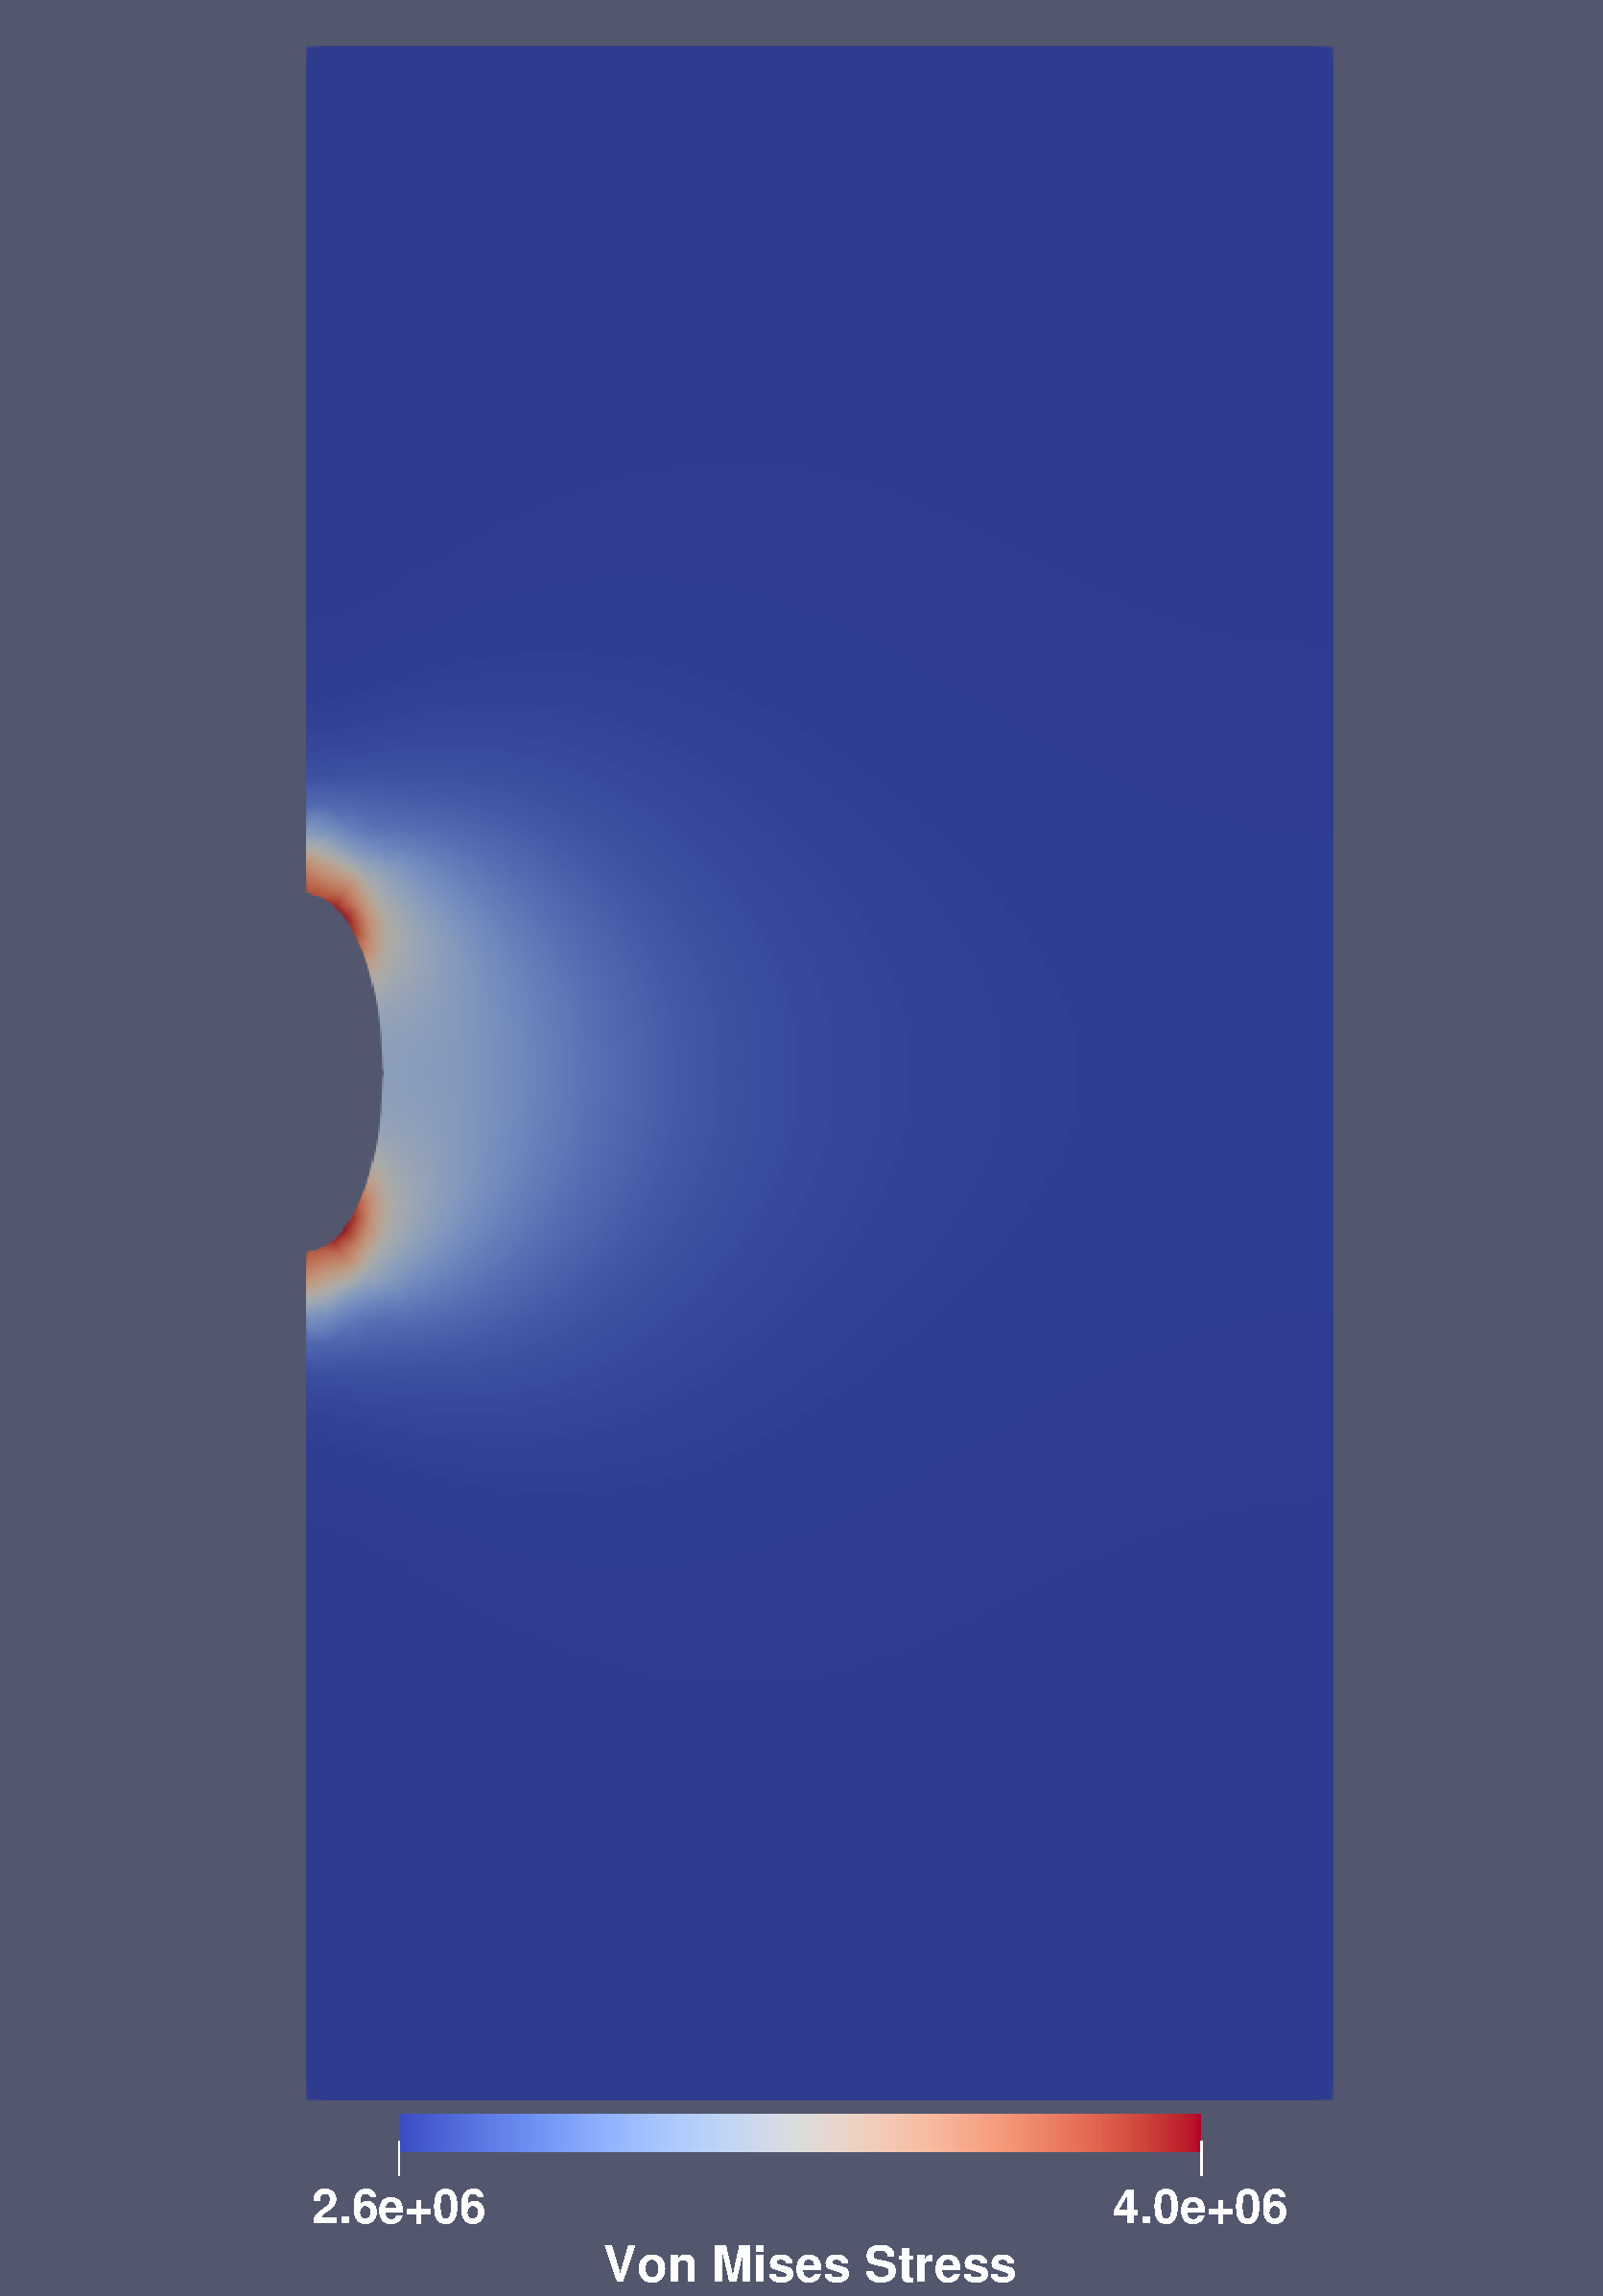
\includegraphics[width=0.95\textwidth]{img/chap4/35mises.pdf}
        \end{minipage}
    }
    \subfigure[90℃~Mises应力云图]
    {
        \begin{minipage}{7cm}
            \centering
            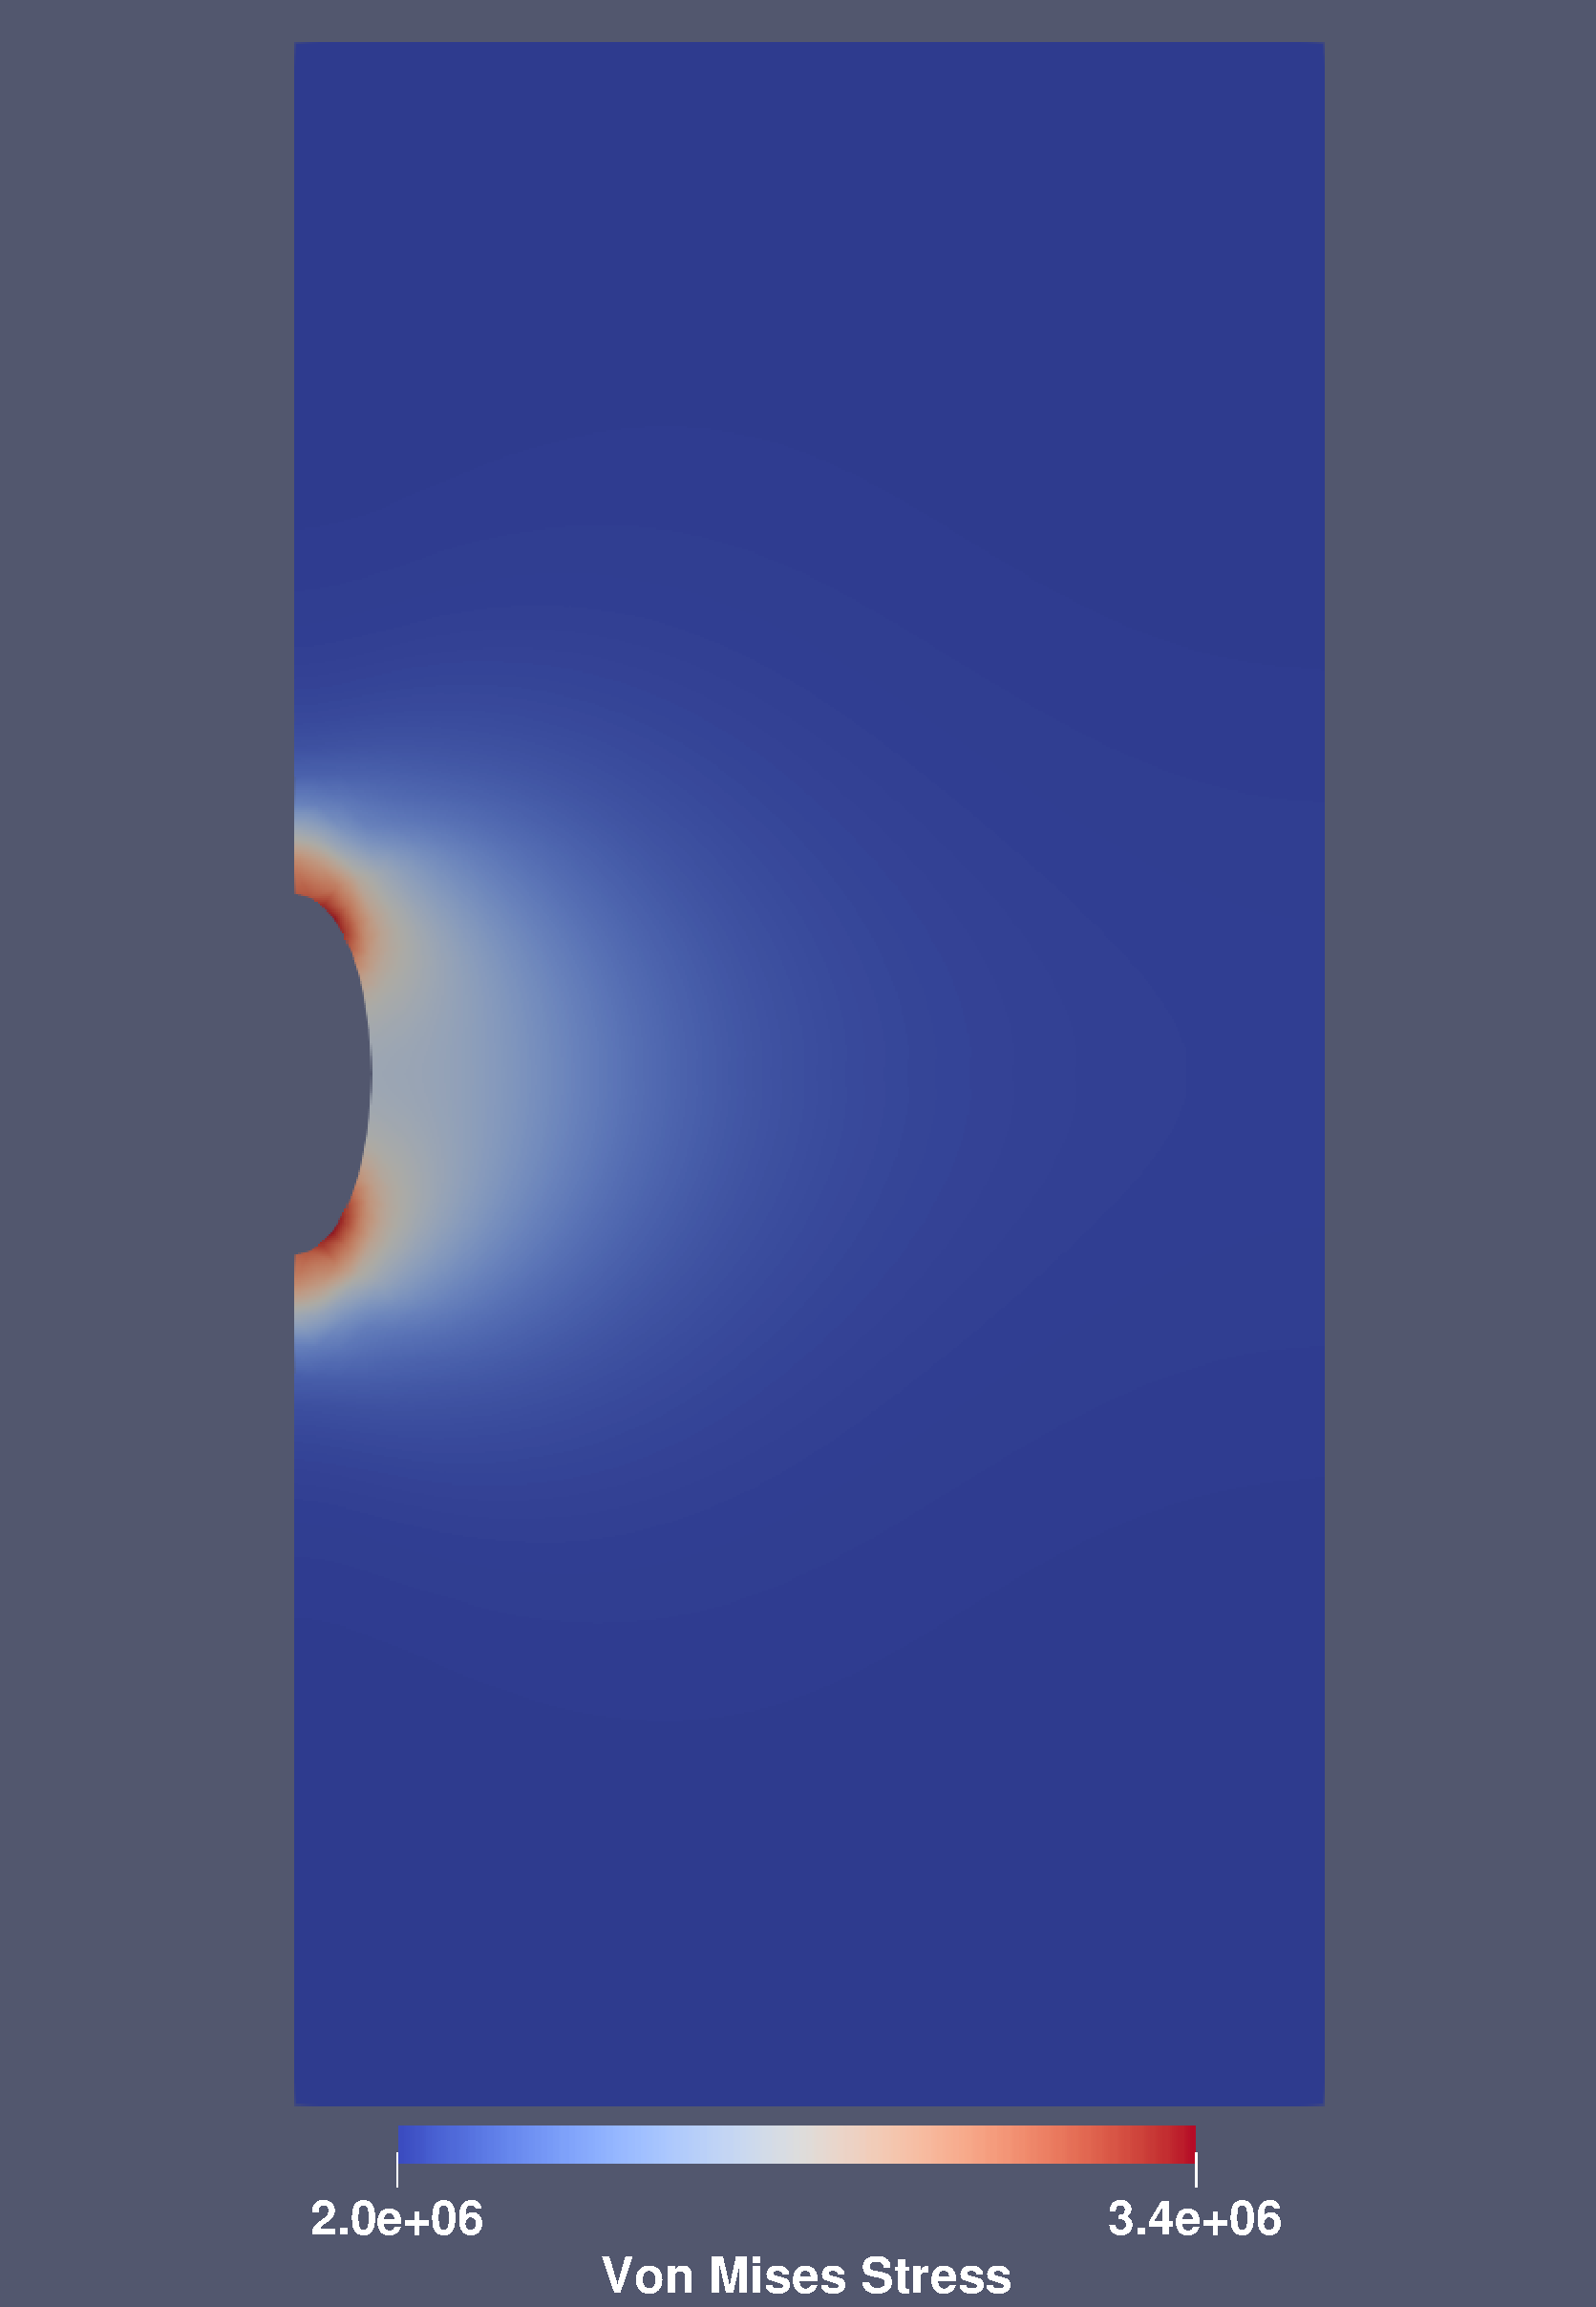
\includegraphics[width=0.95\textwidth]{img/chap4/90mises.pdf}
        \end{minipage}
    }
    \subfigure[150℃~Mises应力云图]
    {
        \begin{minipage}{7cm}
            \centering
            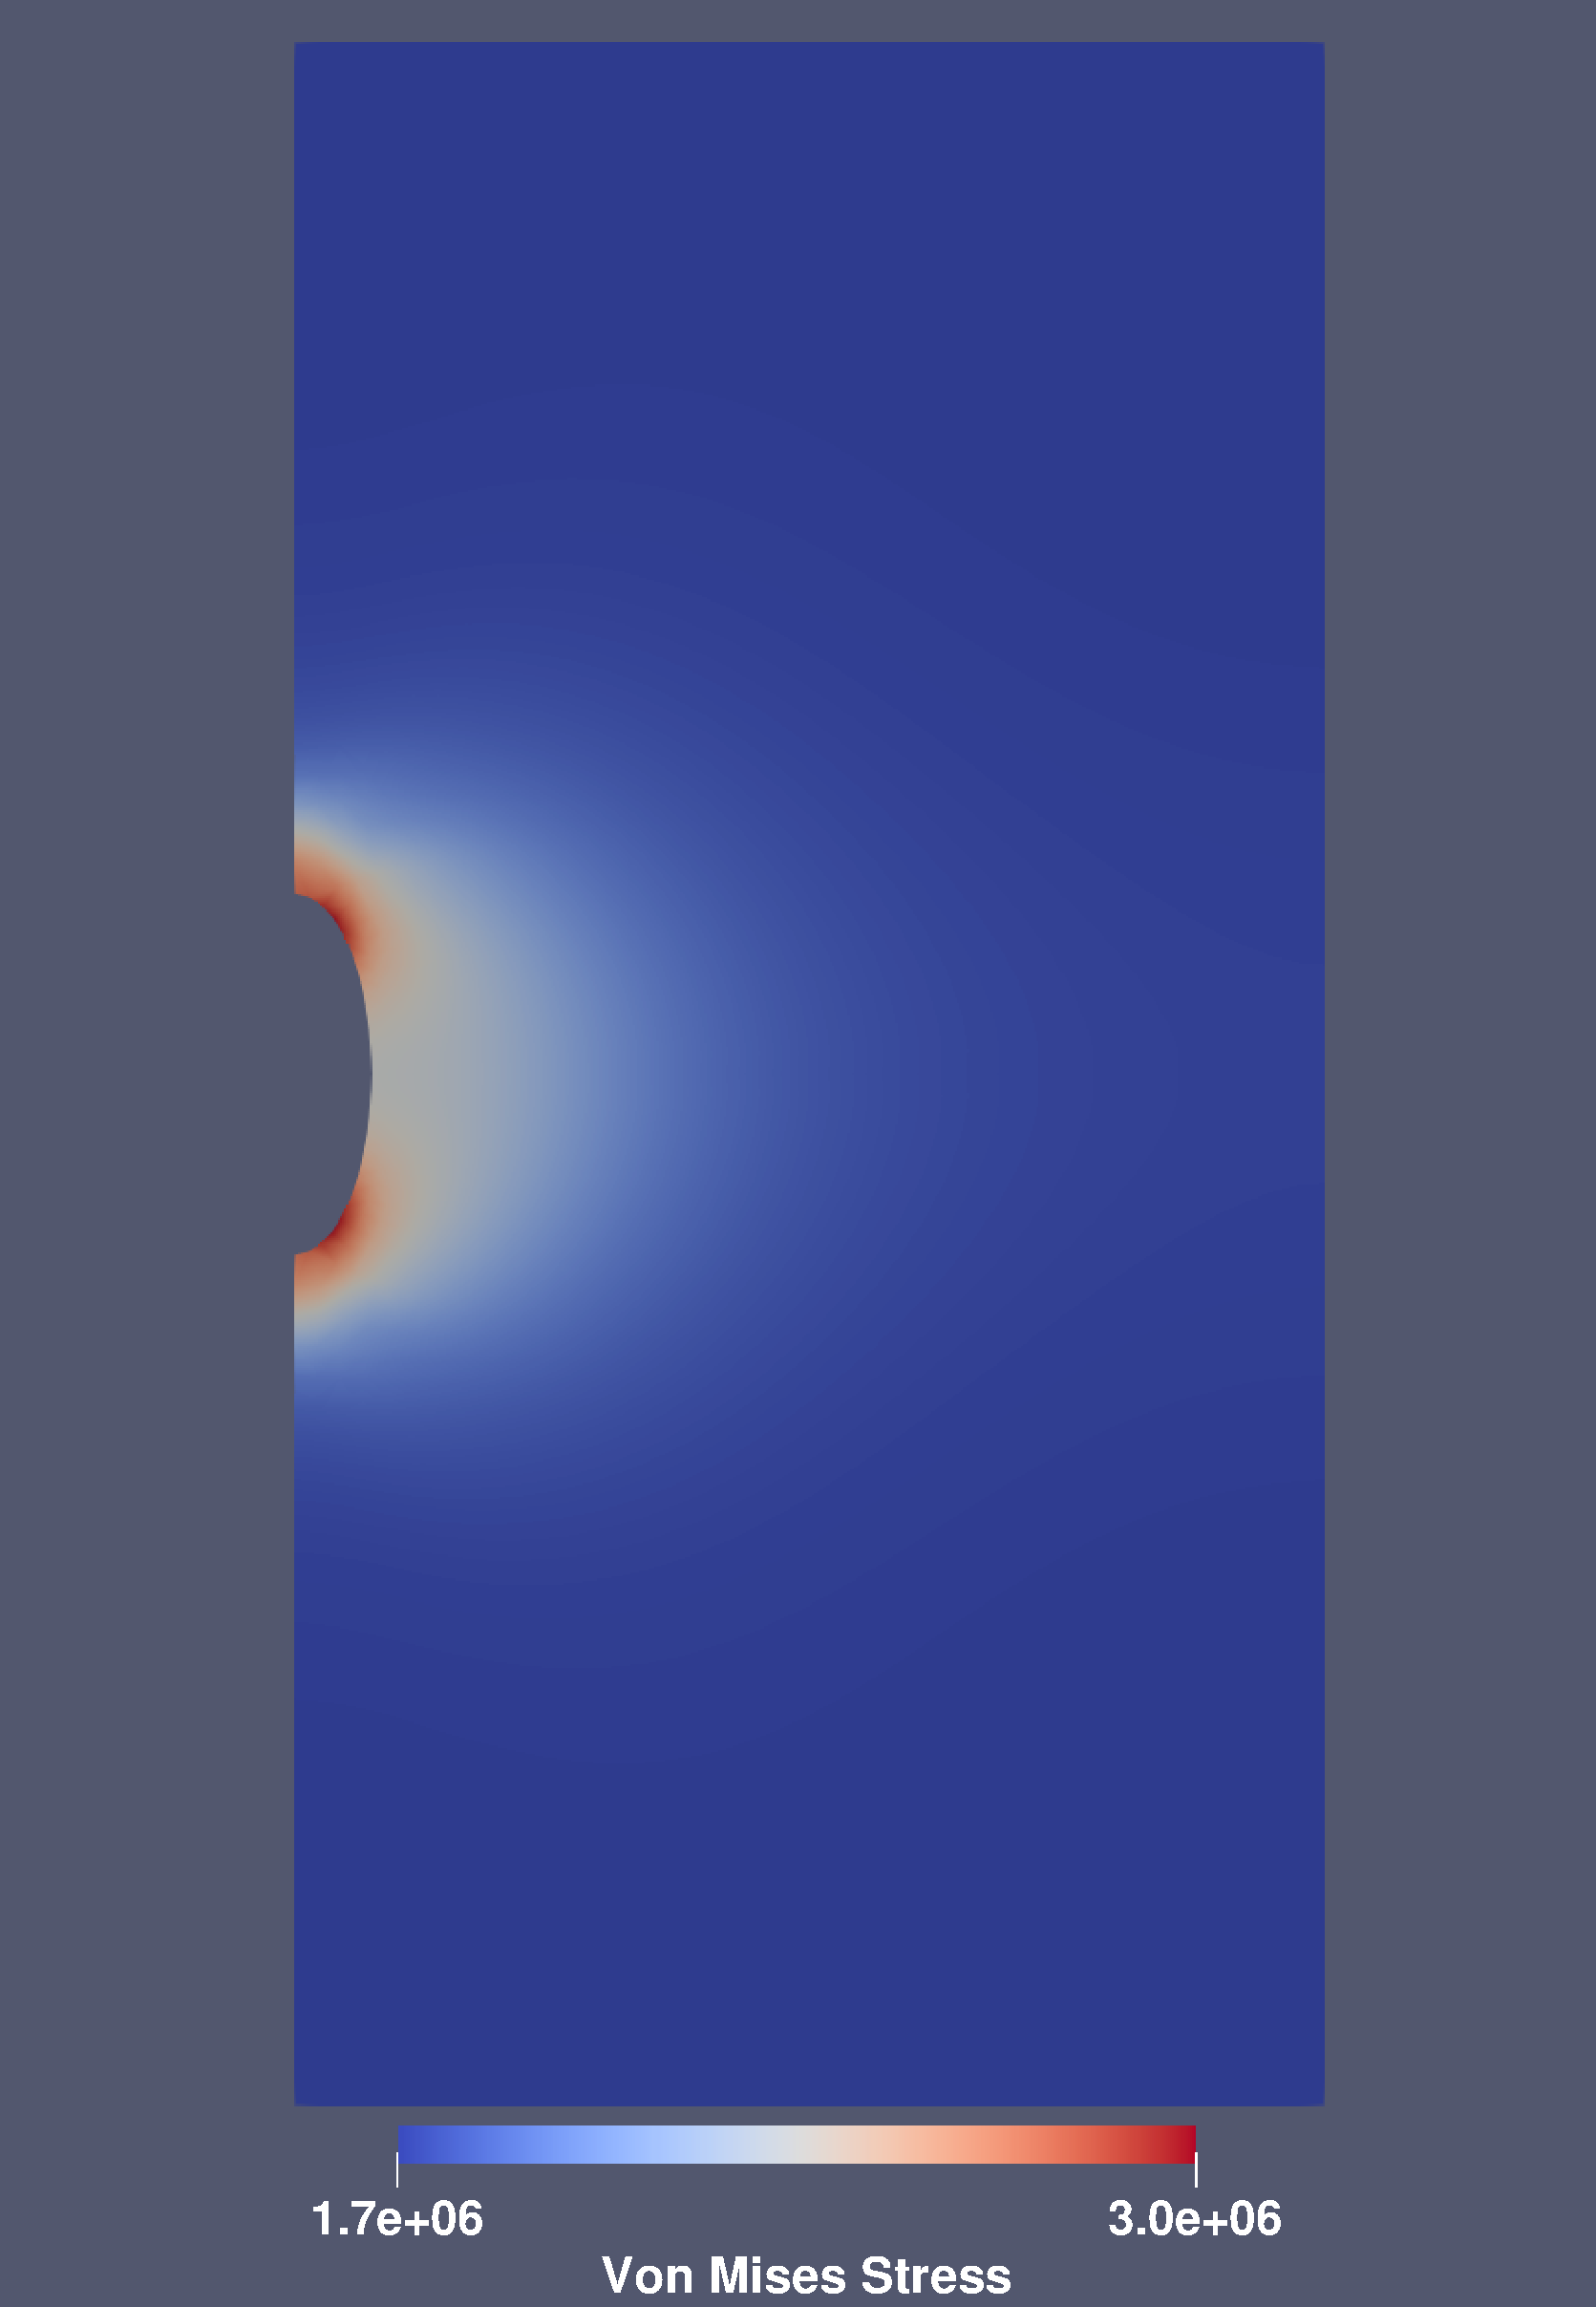
\includegraphics[width=0.95\textwidth]{img/chap4/150mises.pdf}
        \end{minipage}
    }
    \caption{不同温度下Mises应力云图(单位:Pa)}
    \label{fig:Mises}
\end{figure}


\section{小结}

本章从地理位置、自然条件、地址条件等方面介绍了金坛盐矿的工程地质概况,重点阐述了金坛地区的盐岩层地质特征。并建立二维数值模型,编写OpenGeoSys计算脚本进行计算,得到了围岩的位移场、应力场随时间的变化情况。分析结果发现:(1)温度越高,围岩产生的最大位移越大;(2)盐岩储库呈现明显的初始蠕变和稳态蠕变特征;(3)围岩位移集中于腔腰,应力集中于腔顶和腔底。结论符合盐岩的力学特性、温度对盐岩蠕变影响规律,符合椭球形腔体的破坏特点,因此可校验计算方法和计算输入文件的合理性。